\documentclass[a4paper,english,11pt,twoside]{article}
\usepackage[utf8]{inputenc}
\usepackage[T1]{fontenc}
\usepackage[english]{babel}
\usepackage{epsfig}
\usepackage{graphicx}
\usepackage{amsmath}
\usepackage{pstricks}
\usepackage{subcaption}
\usepackage{booktabs}
\usepackage{float}
\usepackage{gensymb}
\usepackage{preamble}
\usepackage{movie15}
\restylefloat{table}
\renewcommand{\arraystretch}{1.5}
 \newcommand{\tab}{\hspace*{2em}}


\date{\today}
\title{Mandatory Assignment 1}
\author{Jørgen D. Tyvand}

\begin{document}
\maketitle
\newpage

\section*{1)}
(The following description of pisoFoam is largely based on the description given on openfoamwiki.net)\\
\\
The basic structure of the piso algorithm as implemented in pisoFoam is as follows:\\
\\
$\mathbf{Step 1}$: Boundary conditions are set\\
\\
$\mathbf{Step 2}$: The discretized momentum equation is defined and solved:\\
\begin{lstlisting}[style=python]
fvVectorMatrix UEqn
(
   fvm::ddt(U)
   + fvm::div(phi, U)
   + turbulence->divDevReff(U)
 );
\end{lstlisting}
This equation differs in my version of OpenFoam from the one given for pisoFoam at openfoamwiki.net and Chalmers in the final term, where the other sources gives\\
\begin{lstlisting}[style=python]
 fvVectorMatrix UEqn
 (
   fvm::ddt(U)
   + fvm::div(phi, U)
   - fvm::laplacian(nu,Step 2 U)
 );
\end{lstlisting}
The final term in my version, as i understand, is a combination of a laplacian and the divergence of the deviatoric  (the deviatoric being the difference between the Cauchy stress tensor and the hydrostatic stress tensor)
\begin{lstlisting}[style=python]
divDevReff(U) =
- fvm::laplacian(nuEff(), U)
- fvc::div(nuEff()*dev(fvc::grad(U)().T())) 
\end{lstlisting}
We then solve the equation
\begin{lstlisting}[style=python]
solve(UEqn == -fvc::grad(p));
\end{lstlisting}
\newpage
$\mathbf{Step 3}$: The piso loop then starts, begining with calculating the coefficients and the flux
\begin{lstlisting}[style=python]
 volScalarField rAU(1.0/UEqn.A());

volVectorField HbyA("HbyA", U);
HbyA = rAU*UEqn.H();
surfaceScalarField phiHbyA
 (
   "phiHbyA",
   (fvc::interpolate(HbyA) & mesh.Sf())
   + fvc::interpolate(rAU)*fvc::ddtCorr(U, phi)
);

adjustPhi(phiHbyA, U, p);
\end{lstlisting}
$\mathbf{Step 4}$: The pressure equation is solved
\begin{lstlisting}[style=python]
fvScalarMatrix pEqn
 (
   fvm::laplacian(rAU, p) == fvc::div(phiHbyA)
 );

pEqn.setReference(pRefCell, pRefValue);
\end{lstlisting}
In this case, the nNonOrthCorr is set to 0, so there are no non-orthogonal pressure corrections.\\
\\
$\mathbf{Step 5}$: The velocites and boundary conditions are corrected
\begin{lstlisting}[style=python]
 U = HbyA - rAU*fvc::grad(p);
U.correctBoundaryConditions();
\end{lstlisting}
$\mathbf{Step 6}$: The loop is repeated the number of times given by nCorrectors in the fvSolution file.\\
\\
$\mathbf{Step 7}$: The time step is increased and the process starts again from step 1.
\section*{2)}
For both the LES and RANS models, we start from the Navier-Stokes equations for incompressible flow:\\
\\
$\nabla\cdot (\rho\vec{u}) = 0$\\
\\
$\pdi{(\rho u)}{t} + \nabla\cdot(\rho u \vec{u}) = -\pdi{p}{x} + \mu\nabla^2u$\\
\\
$\pdi{(\rho v)}{t} + \nabla\cdot(\rho v \vec{u}) = -\pdi{p}{y} + \mu\nabla^2v$\\
\\
Lengthy derivations of the LES and RANS equations will not be given, but a short explanation of each will give the general process.\\
\\
For Large Eddy Simulation (LES), we use spatial filtering to separate varying sizes of eddies. A cutoff width $\Delta$ is introduced, for which information about eddies smaller than the given width will be ignored/destroyed. A spatial filtering using a filter finction $G(\vec{x},\vec{x}', \Delta)$ is introduced, giving in the following form (3.84 in the book):\\
\\
$\ol\phi(\vec{x},t) \equiv \displaystyle\int\limits_{-\infty}^\infty\int\limits_{-\infty}^\infty\int\limits_{-\infty}^\infty\, G(\vec{x},\vec{x}', \Delta)\phi(\vec{x}', t)\mathrm dx_1'\mathrm dx_2'\mathrm dx_3'$\\
\\
where $\ol\phi(\vec{x},t)$ and $\phi(\vec{x}, t)$ are the filtered and unfiltered functions respectively. The filter function $G(\vec{x},\vec{x}', \Delta)$ can be given in several ways, but the one used in finite volume implementations is the top-hat/box filter function\\
\\
$
 G(\vec{x},\vec{x}', \Delta) = 
  \begin{cases} 
   \frac{1}{\Delta^3} & \abs{\vec{x} - \vec{x}'} \leq \Delta / 2 \\
   0       & \abs{\vec{x} - \vec{x}'} > \Delta / 2
  \end{cases}
$\\
\\
Using this filtering on the Navier-Stokes equations, we get the LES momentum equations (the intermediate step from 3.88a-c to 3.89a-c in the book for rewriting the term $\nabla\cdot(\rho\ol{\phi\vec{u}})$ is not shown):\\
\\
$\pdi{(\rho \ol{u})}{t} + \nabla\cdot(\rho \ol{u}\, \vec{\ol{u}}) = -\pdi{\ol{p}}{x} + \mu\nabla^2\ol{u} - (\nabla\cdot(\rho \ol{u\vec{u}}) - \nabla\cdot(\rho \ol{u}\, \vec{\ol{u}}))$\\
\\
$\pdi{(\rho \ol{v})}{t} + \nabla\cdot(\rho \ol{v}\, \vec{\ol{u}}) = -\pdi{\ol{p}}{y} + \mu\nabla^2\ol{v} - (\nabla\cdot(\rho \ol{v\vec{u}}) - \nabla\cdot(\rho \ol{v}\, \vec{\ol{u}}))$\\
\\
The boundary conditions for the LES problem is as following:\\
\\
Uniform velocity of 10 m/s in the x-direction at the inlet\\
Zero velocity gradient at the walls and outlet\\
Zero pressure gradient at the walls and inlet\\
A uniform value of 0 for the pressure at the outlet\\
\\
For the simulations i have used 2 different mesh refinements, one with 10x20 cells for the inlet and outlet boxes and 100x20 for the center boxes, as well as a doubled mesh of 20x40 and 200x40 boxes. The case files were originally copied from the PitzDaily case for incompressible flow with PISO, and edited from there. For the convection term i have tested different upwind schemes, and landed on filteredLinear. An upwind scheme will include more information from upwind cells, and therefore (hopefully) give a more correct and stable calculation. I have tested the following 4 schemes for the coarsest mesh:\\
\\
Non-upwind linear (as found in the unaltered PitzDaily files)\\
upwind\\
linearUpwind\\
filteredLinear\\
\newpage
The following four movie files shows a simulation of these four schemes for 0.5 seconds on the 100 mesh:\\
\begin{figure}[h!]
	\begin{subfigure}{0.2\textwidth}
		\includemovie[poster,]{4cm}{4cm}{animation_piso_10.mp4}
		\caption{$\mathbf{linear}$}
 	\end{subfigure}
	\begin{subfigure}{0.2\textwidth}
		\includemovie[poster,]{4cm}{4cm}{animation_piso_10_upwind.mp4}
		\caption{$\mathbf{upwind}$}
 	\end{subfigure}
	\begin{subfigure}{0.2\textwidth}
		\includemovie[poster,]{4cm}{4cm}{animation_piso_10_linear_upwind.mp4}
		\caption{$\mathbf{upwindLinear}$}
 	\end{subfigure}
	\begin{subfigure}{0.2\textwidth}
		\includemovie[poster,]{4cm}{4cm}{animation_piso_10_filteredLinear.mp4}
		\caption{$\mathbf{filteredLinear}$}
 	\end{subfigure}
\end{figure}

The filteredLinear scheme has also been used for the 200 mesh, as well as a even finer mesh of 250x50 central boxes. As we can see from the following videos, the solutions are mot mesh independent\\
\begin{figure}[h!]
	\begin{subfigure}{0.5\textwidth}
		\includemovie[poster,]{4cm}{4cm}{animation_piso_20_filteredLinear.mp4}
		\caption{$\mathbf{filteredLinear, 200-mesh}$}
 	\end{subfigure}
	\begin{subfigure}{0.5\textwidth}
		\includemovie[poster,]{4cm}{4cm}{animation_piso_25_filteredLinear.mp4}
		\caption{$\mathbf{filteredLinear, 250-mesh}$}
 	\end{subfigure}
\end{figure}
\\
I also found that the solver crashed if i used a too fine mesh with a too coarse time step. In the final calculations i have used timesteps of $1.0*10^{-5}$, but with a timestep of $1.0*10^{-4}$ the Courant number grew to between 1.5 and 2, at which the calculations crashed. This implies grid sensitivity with respect to grid size and time step size.\\
\newpage
Finally we have the mean velocity and mean pressure for the 100, 200- and 250-meshes (at time 0.5 s)\\
\begin{figure}[h!]
	\begin{subfigure}{0.3\textwidth}
		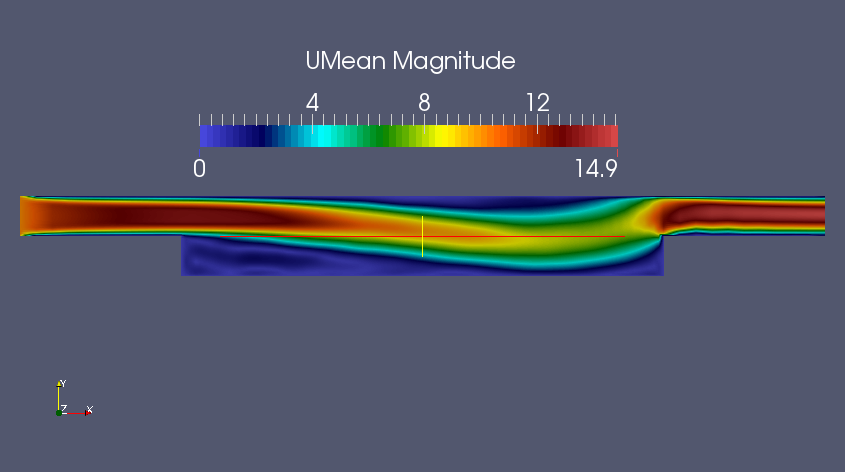
\includegraphics[width=0.95\linewidth]{piso_10_filteredLinear_mean_u.png}
		\caption{$\mathbf{100-mesh}$}
	\end{subfigure}
	\begin{subfigure}{0.3\textwidth}
		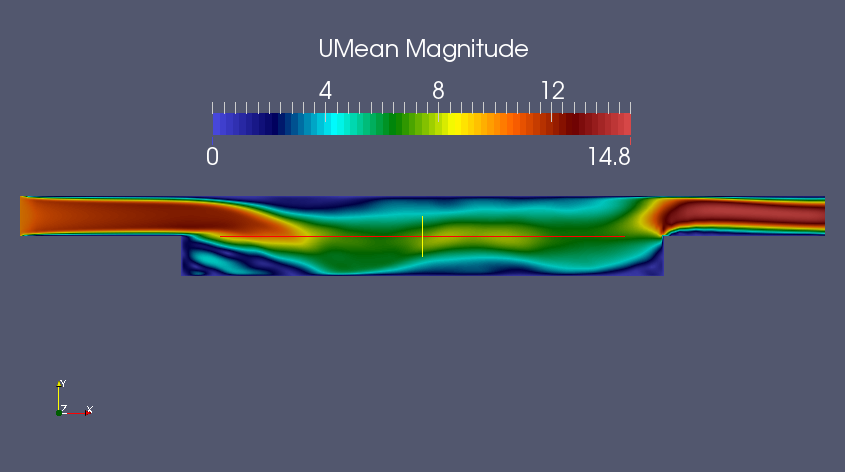
\includegraphics[width=0.95\linewidth]{piso_20_filteredLinear_mean_u.png}
		\caption{$\mathbf{200-mesh}$}
	\end{subfigure}
	\begin{subfigure}{0.3\textwidth}
		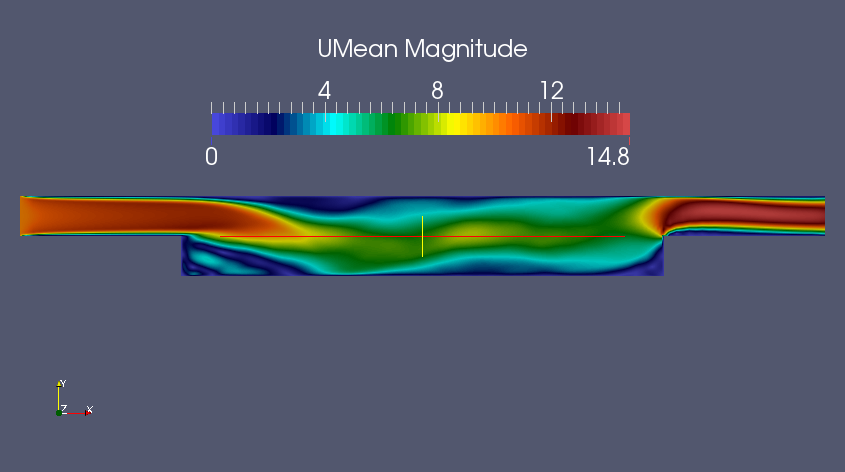
\includegraphics[width=0.95\linewidth]{piso_25_filteredLinear_mean_u.png}
		\caption{$\mathbf{250-mesh}$}
	\end{subfigure}
\end{figure}\\
\begin{figure}[h!]
	\begin{subfigure}{0.3\textwidth}
		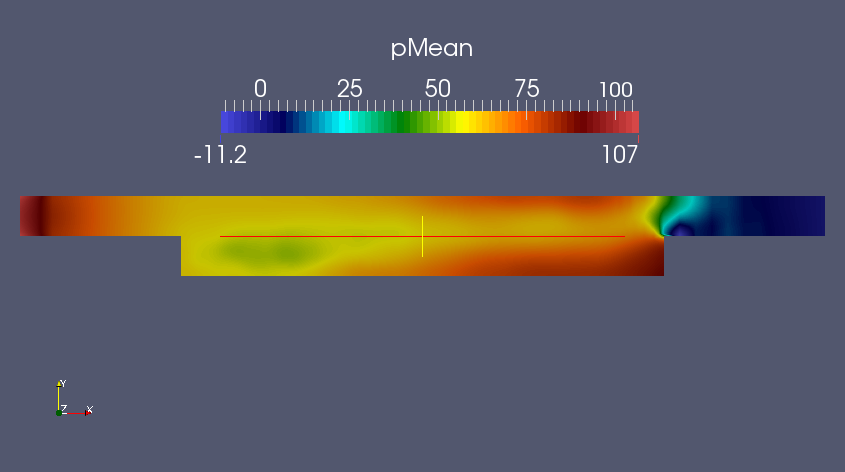
\includegraphics[width=0.95\linewidth]{piso_10_filteredLinear_mean_p.png}
		\caption{$\mathbf{100-mesh}$}
	\end{subfigure}
	\begin{subfigure}{0.3\textwidth}
		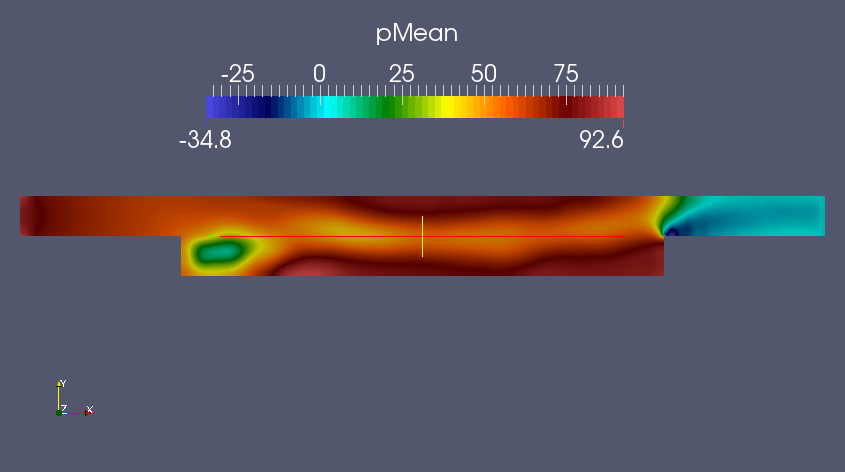
\includegraphics[width=0.95\linewidth]{piso_20_filteredLinear_mean_p.png}
		\caption{$\mathbf{200-mesh}$}
	\end{subfigure}
	\begin{subfigure}{0.3\textwidth}
		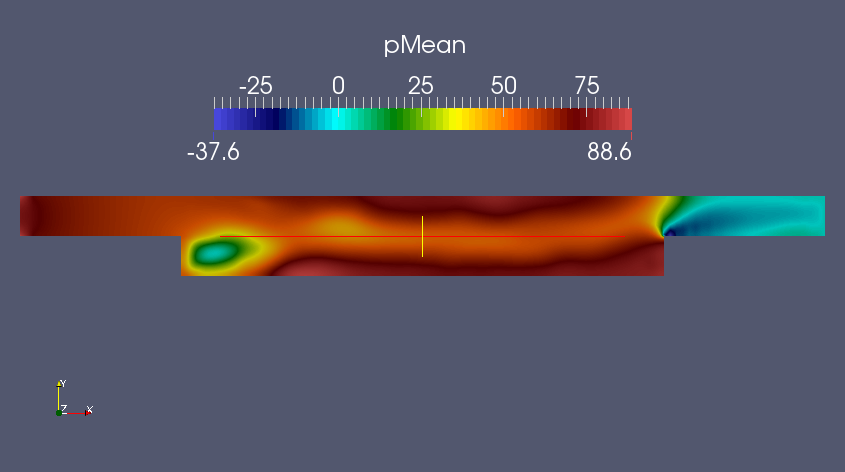
\includegraphics[width=0.95\linewidth]{piso_25_filteredLinear_mean_p.png}
		\caption{$\mathbf{250-mesh}$}
	\end{subfigure}
\end{figure}\\
\\
As we can see, there is more consistency between the mesh sizes for the mean velocity and pressure, but still the differences are noticeable.
\section*{3)}
For the RANS models i have chosen to use the simpleFoam solver for the $k-\epsilon$ and $k-\omega$ models. The general RANS equations are as follows:\\
\\
$\nabla\cdot\vec{\ol{u}} = 0$\\
\\
$\pdi{\ol{u}}{t} + \nabla\cdot(\ol{u}\vec{\ol{u}}) = -\frac{1}{\rho}\pdi{\ol{p}}{x} + \nu\nabla^2\ol{u} + \frac{1}{\rho}\left[\pdi{(-\rho\ol{u'^2})}{x} + \pdi{(-\rho\ol{u'v'})}{y} + \pdi{(-\rho\ol{u'w'})}{z}\right]$
\\
\\
$\pdi{\ol{v}}{t} + \nabla\cdot(\ol{v}\vec{\ol{u}}) = -\frac{1}{\rho}\pdi{\ol{p}}{y} + \nu\nabla^2\ol{v} + \frac{1}{\rho}\left[\pdi{(-\rho\ol{u'v'})}{x} + \pdi{(-\rho\ol{v'^2})}{y} + \pdi{(-\rho\ol{v'w'})}{z}\right]$
\\
\\
$\pdi{\ol{w}}{t} + \nabla\cdot(\ol{w}\vec{\ol{u}}) = -\frac{1}{\rho}\pdi{\ol{p}}{z} + \nu\nabla^2\ol{w} + \frac{1}{\rho}\left[\pdi{(-\rho\ol{u'w'})}{x} + \pdi{(-\rho\ol{v'w'})}{y} + \pdi{(-\rho\ol{w'^2})}{z}\right]$
\\
\\
Here the overline marks the mean terms, and the marked terms are the fluctuation terms. The last bracketed terms in each equation contain the so called Reynolds stresses.\\
\\
For the $k-\epsilon$ model, I have used the value for k that was used in the PitzDaily case, $k = 0.375$. This is because the inlet velocity is the same, and i have assumed that a similar turbulence intensity is appropriate. Analyzing the value for $\epsilon$ in the PitzDaily case, i found that they have used a value of 0.1 times the inlet opening for the turbulent length scale. I have adjusted my value for $\epsilon$ using the same ratio, giving $\epsilon = 7.547$.\\
\newpage
There are two additional equations to be solved for the $k-\epsilon$ model:\\
\\
$\pdi{\rho k}{t} + \nabla\cdot(\rho k \vec{u}) = \frac{\mu_t}{\sigma_k}\nabla^2k + 2\mu_t S_{ij}\cdot S_{ij} - \rho\epsilon$\\
\\
$\pdi{\rho \epsilon}{t} + \nabla\cdot(\rho \epsilon \vec{u}) = \frac{\mu_t}{\sigma_{\epsilon}}\nabla^2\epsilon + C_{1\epsilon}\frac{\epsilon}{k}2\mu_t S_{ij}\cdot S_{ij} - C_{2\epsilon}\rho\frac{\epsilon^2}{k}$\\
\\
Here, $S_{ij}$ are the components of the mean of the rate of deformation. The constants have the following given values (found both in the book and in other sources):\\
\\
$\mu_t = \rho C_{\mu}\frac{k^2}{\epsilon}\tab C_{\mu} = 0.09\tab\sigma_k = 1.00\tab\sigma_{\epsilon} = 1.30\tab C_{1\epsilon} = 1.44\tab C_{2\epsilon} = 1.92$
\\
\\
Running the $k-\epsilon$ case, i have found the following converged solutions for the flow, using the 100 and 200 meshes respectively:\\
\\
The following figures show the mean velocity for the two mesh sizes:\\
\begin{figure}[h!]
	\begin{subfigure}{0.5\textwidth}
		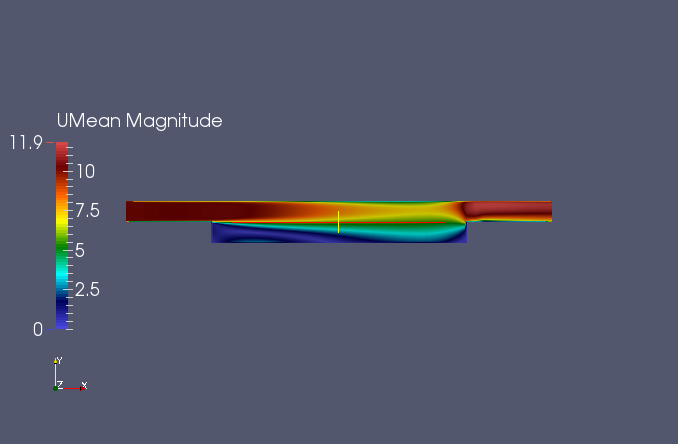
\includegraphics[width=0.95\linewidth]{simple_ke_10_mean_u.png}
		\caption{$\mathbf{ 100-mesh, k-\epsilon}$}
	\end{subfigure}
	\begin{subfigure}{0.5\textwidth}
		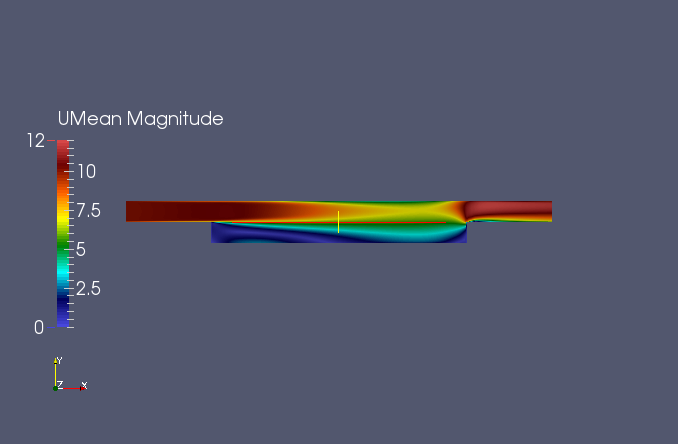
\includegraphics[width=0.95\linewidth]{simple_ke_20_mean_u.png}
		\caption{$\mathbf{ 200-mesh, k-\epsilon}$}
	\end{subfigure}
\end{figure}
\\
And finally we have the mean kinematic energy:\\
\begin{figure}[h!]
	\begin{subfigure}{0.5\textwidth}
		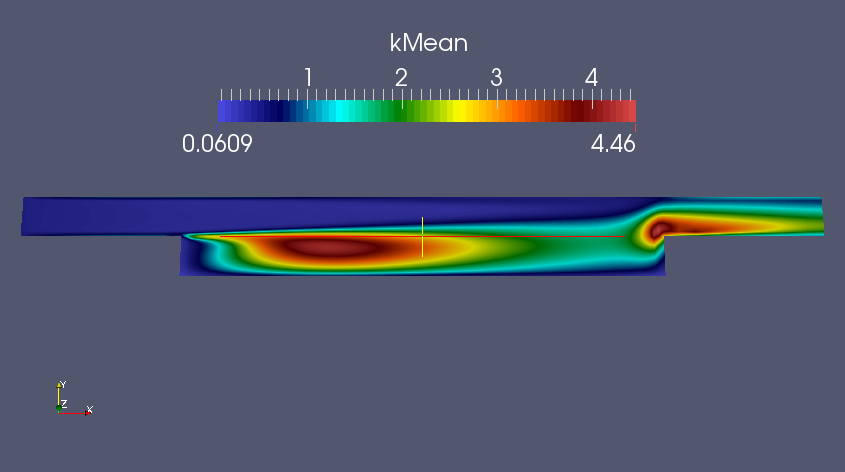
\includegraphics[width=0.95\linewidth]{simple_ke_10_mean_k.png}
		\caption{$\mathbf{ 100-mesh, k-\omega}$}
	\end{subfigure}
	\begin{subfigure}{0.5\textwidth}
		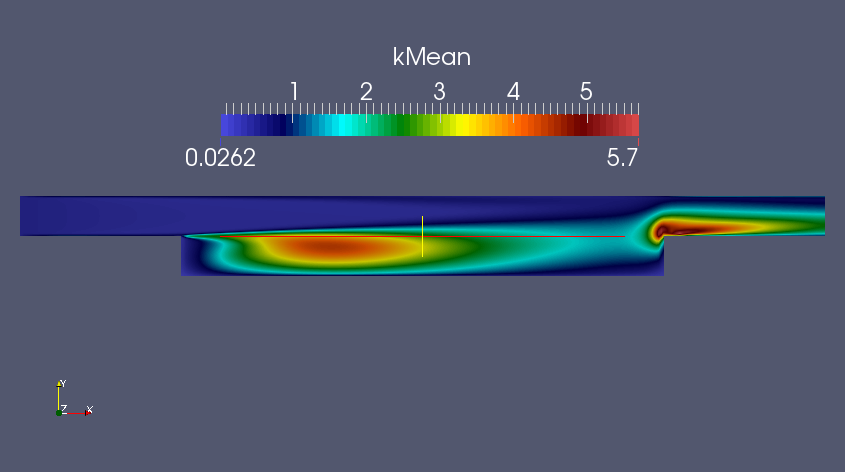
\includegraphics[width=0.95\linewidth]{simple_ke_20_mean_k.png}
		\caption{$\mathbf{ 200-mesh, k-\omega}$}
	\end{subfigure}
\end{figure}
\\
We see that there is just a slight difference between the two cases, so there is little or no mesh sensitivity using simpleFoam for this RANS problem.\\
\newpage
For the $k-\omega$ model, i have used the fact that $\omega = \frac{\epsilon}{k}$, and used the values from the $k-\epsilon$ problem to calculate $\omega = 20.125$. We have two additional equations in this model as well:\\
\\
$\pdi{\rho k}{t} + \nabla\cdot(\rho k \vec{u}) = (\mu + \frac{\mu_t}{\sigma_k})\nabla^2k + P_k - \beta^*\rho k\omega\tab P_k = \left(2\mu_t S_{ij}\cdot S_{ij} - \frac{2}{3}\rho k\pdi{U_i}{x_j}\delta_{ij}\right)$\\
\\
$\pdi{\rho \omega}{t} + \nabla\cdot(\rho \omega \vec{u}) = (\mu + \frac{\mu_t}{\sigma_{\omega}})\nabla^2\omega + \gamma_i\left(2\rho S_{ij}\cdot S_{ij} - \frac{2}{3}\rho \omega\pdi{U_i}{x_j}\delta_{ij}\right) - \beta_1\rho\omega^2$\\
\\
With constants\\
\\
$\sigma_k = 2.0\tab\sigma_{\omega} = 2.0\tab\gamma_1 = 0.553\tab\beta_1 = 0.075\tab\beta^* = 0.09$\\
\\
Running simpleFoam, we get the following plots for the converged values of the mean velocity for the 100 and 200 meshes:\\
\begin{figure}[h!]
	\begin{subfigure}{0.5\textwidth}
		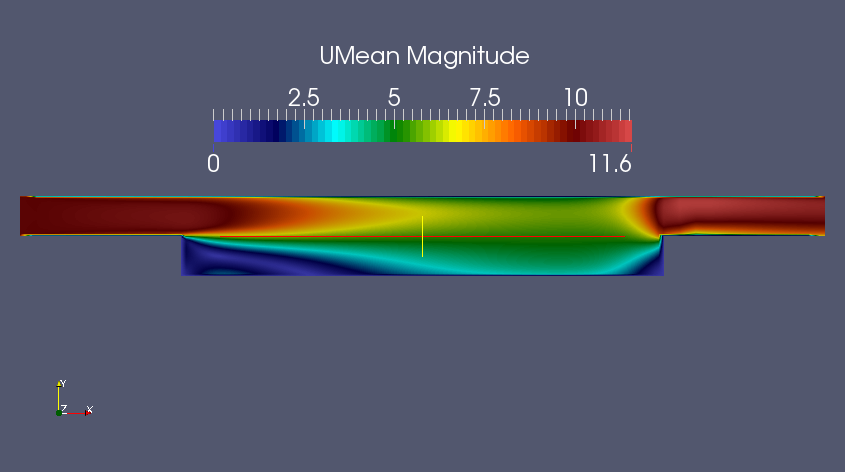
\includegraphics[width=0.95\linewidth]{simple_ko_10_mean_u.png}
		\caption{$\mathbf{ 100-mesh, k-\epsilon}$}
	\end{subfigure}
	\begin{subfigure}{0.5\textwidth}
		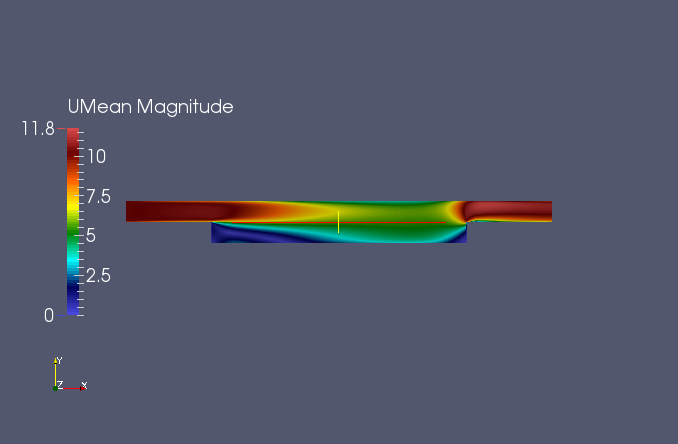
\includegraphics[width=0.95\linewidth]{simple_ko_20_mean_u.png}
		\caption{$\mathbf{ 200-mesh, k-\epsilon}$}
	\end{subfigure}
\end{figure}
\\
And for the mean kinematic energy:\\
\begin{figure}[h!]
	\begin{subfigure}{0.5\textwidth}
		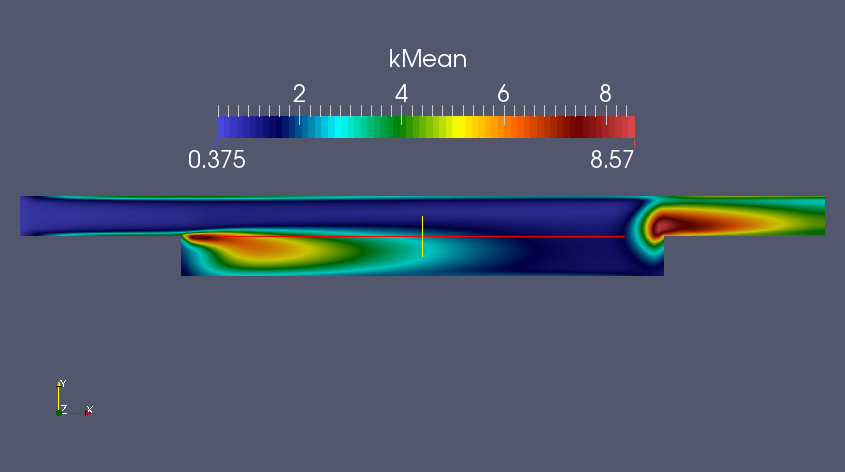
\includegraphics[width=0.95\linewidth]{simple_ko_10_mean_k.png}
		\caption{$\mathbf{ 100-mesh, k-\omega}$}
	\end{subfigure}
	\begin{subfigure}{0.5\textwidth}
		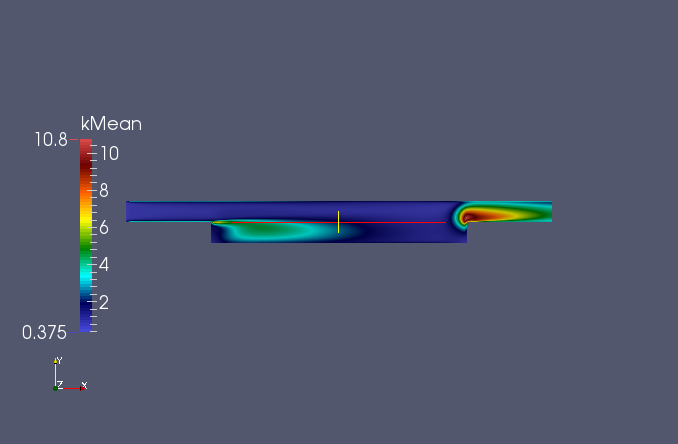
\includegraphics[width=0.95\linewidth]{simple_ko_20_mean_k.png}
		\caption{$\mathbf{ 200-mesh, k-\omega}$}
	\end{subfigure}
\end{figure}
\\
\section*{4)}
Since pimpleFoam is a large time-step solver, i would assume that some of the eddy information would be lost in a LES model if the pimpleFoam solver incorporates time step adjustments as I have found to appear in some of the pimpleFoam tutorial cases' controlDict files. As some of the eddies appear, travel and dissapear in very short amounts of time, this might not be picked up by the solver using larger than needed time steps.
\section*{5)}
To compare the results from the LES and RANS calculations, i have plotted the streamlines at the last time step (0.5 s) for the 200-mesh solution for the $k-\epsilon$ and $k-\omega$ cases, as well as for the 250-mesh solution for the filteredLinear LES simulation\\
\\
\begin{figure}[h!]
	\begin{subfigure}{0.3\linewidth}
		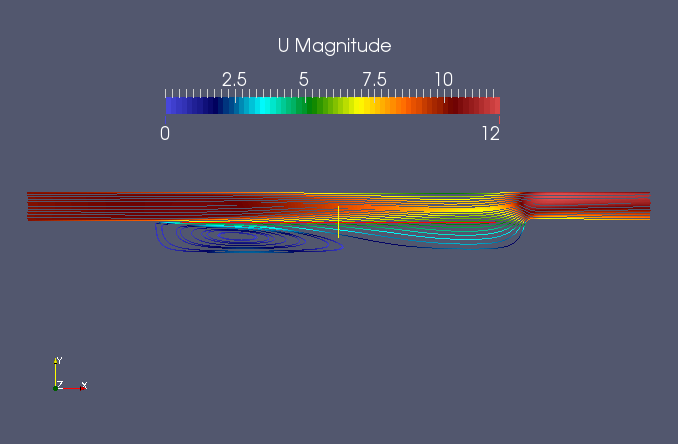
\includegraphics[width=0.95\linewidth]{simple_ke_20_streamlines.png}
		\caption{$\mathbf{k-\epsilon}$}
	\end{subfigure}
	\begin{subfigure}{0.3\linewidth}
		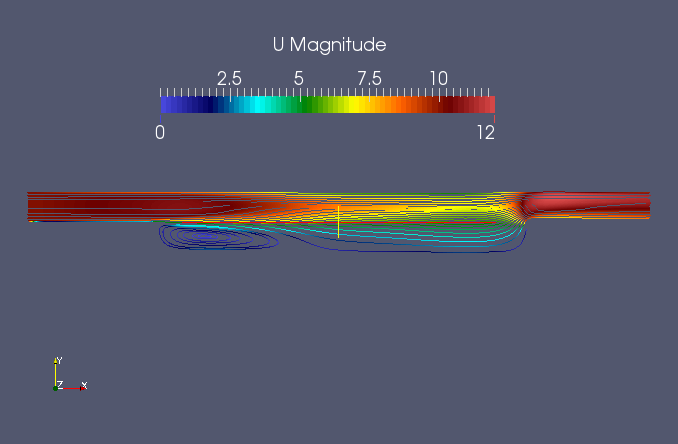
\includegraphics[width=0.95\linewidth]{simple_ko_20_streamlines.png}
		\caption{$\mathbf{k-\epsilon}$}
	\end{subfigure}
	\begin{subfigure}{0.3\linewidth}
		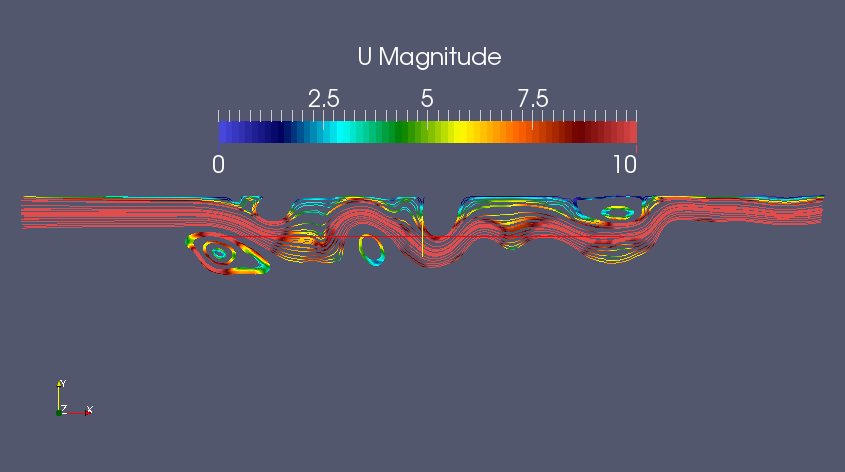
\includegraphics[width=0.95\linewidth]{piso_25_filteredLinear_streamlines.png}
		\caption{$\mathbf{piso}$}
	\end{subfigure}
\end{figure}\\
We can see that the location of the recirculation bubble is roughly the same for all three cases, but the bubble is longer for the$k-\epsilon$ than the $k-\omega$. The location in the LES case shifts through time (as can be seen in the above videos), as well as the generated "bubble" letting go and reappearing several times during the simulation. 
\section*{6)}
Since turbulence is a three-dimensional phenomenon.
 \end{document}
